\chapter{Astroparticle Physics at a Glance}

\begin{flushright}
    \textit{All you really need to know for the moment \\is that the Universe is a lot more complicated than you might think, \\even if you start from a position of thinking it’s pretty damn complicated in the first place.}

    \vspace{0.3cm}
    --- Douglas Adams, \textit{The Hitchhiker's Guide to the Galaxy}
    \vspace{0.3cm}
\end{flushright}

%
\begin{figure}
    \centering
    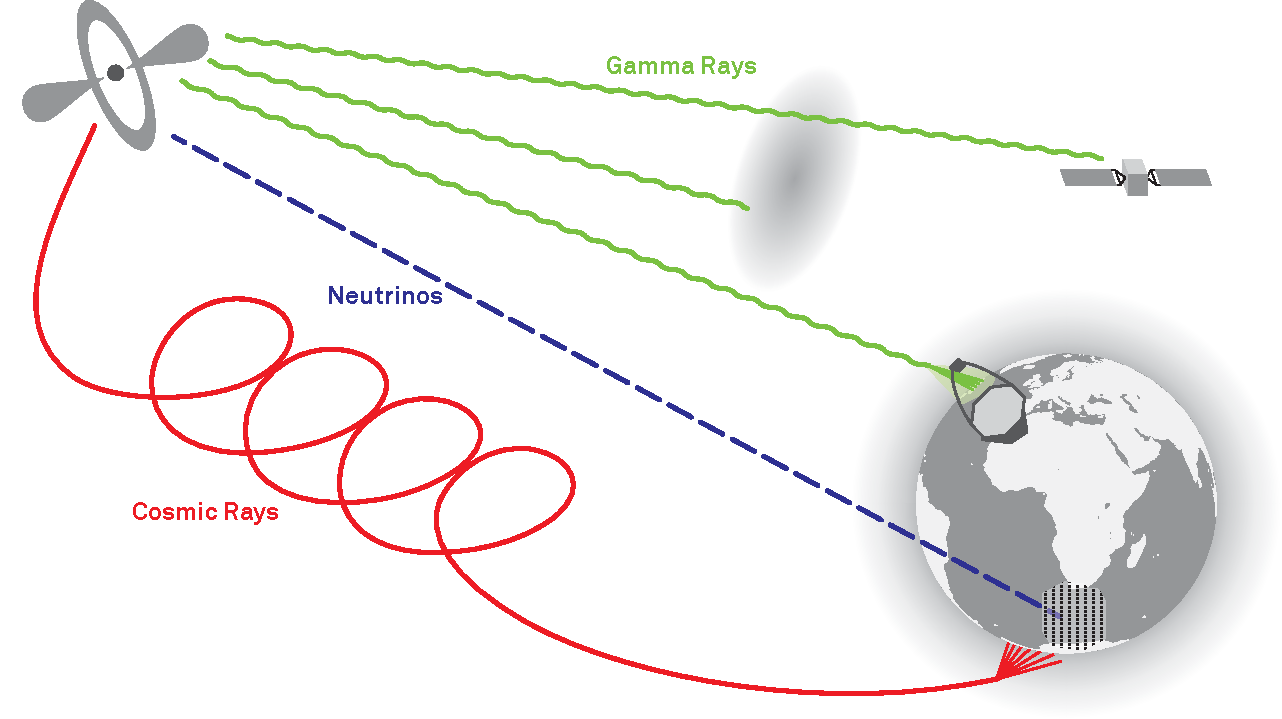
\includegraphics[width=0.9\textwidth]{./figures/agn_earth_messenger.pdf}
    \caption{Astroparticle physics at a glance. Specific astronomical objects emit different messengers, such as neutrinos, cosmic and gamma rays, propagating through the universe. Depending on the type of messenger, they might interact with magnetic fields, interstellar clouds, the Earth's atmosphere or the Earth itself, and they can be detected with different instruments.}
    \label{fig:overview_astro}
\end{figure}
%

\blindtext[4]


